\documentclass{article}

\usepackage{amsmath}
\usepackage{amsthm}
\usepackage{amssymb}
\usepackage{graphicx}

\graphicspath{{pics/}}

%CURLIES  :)       $\{$ $\}$

\newcommand{\ti}[1]{\textit{#1}}
\newcommand{\tb}[1]{\textbf{#1}}
\newcommand{\rn}[1]{\romannum{#1}}
\newcommand{\Rn}[1]{\Romannum{#1}}
\newcommand{\N}{\mathbb{N}}
\newcommand{\Z}{\mathbb{Z}}
\newcommand{\Q}{\mathbb{Q}}
\newcommand{\R}{\mathbb{R}}
\newcommand{\C}{\mathbb{C}}
\newcommand{\Om}{\Omega}
\newcommand{\om}{\omega}
\newcommand{\la}{\lambda}
\newcommand{\ep}{\varepsilon}
\newcommand{\emp}{\emptyset}
\newcommand{\lt}{\textless}
\newcommand{\gt}{\textgreater}
\newcommand{\imply}{\Rightarrow}
\newcommand{\x}{\cdot}
\newcommand{\Ga}{\Gamma}
\newcommand{\al}{\alpha}
\newcommand{\sg}{\sigma}
\newcommand{\be}{\beta}
\newcommand{\de}{\delta}
\newcommand{\prop}{\textbf{Proposition: }}
\newcommand{\thm}{\textbf{Theorem: }}
\newcommand{\lem}{\textbf{Lemma: }}
\newcommand{\cor}{\textbf{Corollary: }}
\newcommand{\proo}{\textbf{Proof: }}
\newcommand{\exx}{\textbf{Example: }}
\newcommand{\exxi}{\textbf{Example 1: }}
\newcommand{\exxii}{\textbf{Example 2:  }}
\newcommand{\exxiii}{\textbf{Example 3:  }}
\newcommand{\soln}{\textbf{Solution: }}
\newcommand{\ds}{\displaystyle}
\newcommand{\floor}[1]{\lfloor #1 \rfloor}
\newcommand{\ceil}[1]{\lceil #1 \rceil}
\newcommand{\bigfloor}[1]{\big\lfloor #1 \big\rfloor}
\newcommand{\bigceil}[1]{\big\lceil #1 \big\rceil}
\newcommand{\Bigfloor}[1]{\Big\lfloor #1 \Big\rfloor}
\newcommand{\Bigceil}[1]{\Big\lceil #1 \Big\rceil}
\newcommand{\biggfloor}[1]{\bigg\lfloor #1 \bigg\rfloor}
\newcommand{\biggceil}[1]{\bigg\lceil #1 \bigg\rceil}
\newcommand{\Biggfloor}[1]{\Bigg\lfloor #1 \Bigg\rfloor}
\newcommand{\Biggceil}[1]{\Bigg\lceil #1 \Bigg\rceil}
\newcommand{\mcal}[1]{\mathcal{#1}}
\newcommand{\bb}[1]{\mathbb{#1}}
\newcommand{\opt}{\text{opt}}

\title{COMP 251: Algorithms \& Data Structures}
\author{Owen Lewis}
\date{Winter 2018}

\begin{document}

\begin{titlepage}
\maketitle
\end{titlepage}

\tableofcontents
\newpage

%%%%%%%%%%%%%%%%%%%%%%%%%%%%%%%%%%%%%%%%%%%%%%%%%%%%%%%%%%%%%%%%%%%%%%%%

\section{Overview of Graph Theory}
\subsection{Definitions}
A graph $G = (V, E)$ is a set $V$ of vertices (a.k.a. nodes) and a set $E$ of edges (denoting vertex pairs). We set $n = |V|$, and $m = |E|$. A graph is said to be \ti{undirected} when for any edge $(u, v) \in E$ there exists an edge $(v, u) \in E$ for some nodes $u$, and $v$. A graph is said to be $\ti{directed}$ if it is not undirected. In other words, the edge set of a directed graph consists of ordered pairs where the edge set of an undirected graph consists of unordered pairs.\\\\
A \ti{walk} is a set of vertices $\{v_0, v_1, \dots, v_{\ell}\}$ such that $(v_i, v_{i+1}) \in E$, $\forall\ 0 \leq i \leq \ell$. 
A walk where $v_0 = v_{\ell}$ is said to be a \ti{circuit} or a \ti{closed walk}.
A circuit where every edge in the graph is used exactly once is known as an \ti{Eulerian circuit}. 
A \ti{cycle} is a walk $\{v_0, v_1, \dots, v_{\ell}\}$ such that every vertex is distinct except $v_0 = v_{\ell}$.
A cycle where every vertex of the graph is used exactly once is known as a \ti{Hamiltonian cycle}.
A walk where every vertex is distinct is said to be a \ti{path}.\\\\
A graph is said to be \ti{connected} if for each $u, v \in V$ there exists a walk from $u$ to $v$.
A graph is said to be \ti{disconnected} id it is not connected.
Each connected subgraph of a graph is called a \ti{component}. A connected graph therefore has exactly one component.\\\\
A connected component with no cycles is called a \ti{tree}. A graph whose components are all trees is said to be a \ti{forrest}. A tree is said to be \ti{spanning} if it contains every vertex in the graph. A vertex in a tree with at most one neighbour is called a \ti{leaf}.\\\\
A \ti{matching} is a set of vertex-disjoint edges i.e. each edge is incident to at most one other edge in a matching. A matching is said to be \ti{perfect} if every vertex is incident to exactly one edge in the matching.\\\\
A \ti{clique} is a set of pairwise adjacent vertices. In \ti{independent set} (a.k.a. a \ti{stable set}) is set of pairwise non-adjacent vertices.\\\\
A \ti{bipartite graph} is a graph such that the vertex set $V$ can be partitioned as $V = X \cup Y$ where each edge has one node in $X$ and the other node in $Y$. Note that $X$ and $Y$ are necessarily independent sets.
\subsection{Some Theorems for Undirected Graphs}
\thm (Handshaking Lemma) Let $G = (V, E)$ be an undirected graph, let $\Ga(v) := \{u : (u, v) \in E\}$ be the set of neighbours of a node $v$, and let the \ti{degree} $\deg(v)$ of a vertex $v$ equal the cardinality of $\Ga(v)$. Then there are an even number of vertices with odd degree.\\
\proo First note that since we're double-counting the number of pairs where $(v, e)$ is an edge incident to $v$
\[2 \x |E| = \sum_{v \in V} \deg(v) \]
Since the degree of a vertex is either even or odd, we can partition $V$ into a set of odd-degree vertices $\mathcal{O}$, and a set of even-degree vertices $\mathcal{E}$. This gives us
\[\sum_{v \in V} \deg(v) = \sum_{v \in \mathcal{O}} \deg(v) + \sum_{v \in \mathcal{E}} \deg(v)\]
which implies
\[\sum_{v \in \mathcal{O}} \deg(v) = 2\x |E| - \sum_{v \in \mathcal{E}} \deg(v)\]
since both the $2\x |E|$ term is even (obvious) and the $\displaystyle \sum_{v \in \mathcal{E}} \deg(v)$ term is even (sum of even numbers) then the $\displaystyle \sum_{v \in \mathcal{O}} \deg(v)$ term must also be even.
\qed\\\\
\thm (Euler's Theorem) If $G$ is an undirected graph then $G$ contains an Eulerian circuit if and only if every vertex has even degree.\\
\proo Easy proof by induction\\\\
\lem A tree $T$ with $n \geq 2$ vertices has at least one leaf vertex.\\
\proo Trees are connected so there exists no vertices with degree 0 when $n \geq 2$. Suppose each vertex has degree of at least 2. Then consider the longest path $P \subseteq T$, $P = \{v_1, v_2, \dots, v_{\ell-1}, v_{\ell}\}$. Since $\deg(v_{\ell}) \geq 2$, $\exists$ a neighbour (of $v_{\ell}$) $x \in P$ with $x \neq v_{\ell-1}$. If $x = v_{\ell + 1}$ then $P$ is not the longest path, a contradiction. Therefore, for $P$ to be the longest path, $x$ must be somewhere else in $P$, but this creates a cycle, another contradiction. Thus there must exist at least one node $v$ such that $0\ \lt\ \deg(v)\ \lt\ 2$ -- a leaf.
\qed\\\\
\thm A tree with $n$ vertices has exactly $n-1$ edges.\\
\proo Simple proof by induction.\\
\ti{Base case:} A tree with one vertex trivially has 0 edges.\\
\ti{Induction Hypothesis:} Assume any tree with $n-1$ vertices has $n-2$ edges.\\
\ti{Inductive Step:} Take a tree with $n \geq 2$ vertices. By the previous lemma this tree contains a leaf vertex $v$. This implies that $T\setminus\{v\}$ is a tree with $n-1$ vertices and by the induction hypothesis $T \setminus \{v\}$ is a tree with $n-2$ edges, which imples that $T$ is a tree with $n-1$ edges.
\qed\\\\
\thm (Hall's Theorem) Let $G = (X \cup Y, E)$ with $|X| = |Y|$ be a bipartite graph. $G$ contains a perfect matching if and only if $\forall\ B \subseteq X$, $|\Ga(B)| \geq |B|$ (Hall's condition).\\
\proo Firstly, the ($\imply$) direction is fairly obvious. If $B \subseteq X$ with $\Ga(B)\ \lt\ |B|$ then the graph can't have a perfect matching. The ($\Leftarrow$) direction is a bit trickier. Suppose Hall's condition is satisfied. Then, take the maximum cardinality matching $M$ is the graph. If $M$ is perfect then we are done. Otherwise there must exist an unmached vertex $b_0$.
\begin{itemize}
	\item Since Hall's condition holds, we have $|\Ga(\{b_0\})| \geq |\{b_{0}\}| = 1$ so $b_0$ must have at least one neighbour $s_0$.
	\item Suppose $s_0$ is matched in $M$ to $b_1$.
	\item Since Hall's condition holds, we have $|\Ga(\{b_0, b_1\})| \geq |\{b_{0}, b_1\}| = 2$ so $\{b_0, b_1\}$ must have at least one neighbour $s_1 \neq s_0$.
	\item Suppose $s_1$ is matched in $M$ to $b_2$.
	\item Since Hall's condition holds, we have $|\Ga(\{b_0, b_1, b_2\})| \geq |\{b_{0}, b_1, b_2\}| = 3$ so $\{b_0, b_1, b_2\}$ must have at least one neighbour $s_2 \notin \{s_0, s_1\}$.
	\item \dots
\end{itemize}
we repeat this argument as long as we can. Since the graph contains a finite number of vertices this process must terminate, but it can only terminate when we reach an unmatched node $s_k$. Using the edges we've formed in $M$ we can create a path $P$ from $b_0$ to $s_k$ that alternates between using non-matching edges and using matching edges. Swapping the matching edges with the non-matching edges gives us one more matching edge (as we have an odd number of edges.) This is still a valid matching as the internal nodes of $P$ are still incident to exactly one matching edge. Also, the end nodes, $b_0$ and $s_k$ were previously unmatched but are now incident to exactly one edge in the new matching. Thus $M$ isn't the maximum capacity matching -- a contradiction.
\qed
\subsection{``````Data Structures'''''' for Representing Graphs}
\subsubsection{Adjacency Matrices}
For a graph, an \ti{adjacency matrix} $M$ is a matrix suxh that
\begin{enumerate}
	\item There is a row for each vertex
	\item There is a column for each vertex
	\item The $ij-th$ entry is defined as $M_{ij} = 
\begin{cases}
1, (i, j) \in E\\
0, (i, j) \notin E
\end{cases}$
\end{enumerate}
Note that in an undirected graph the matric is symmetric around the diagonal because $(i, j) \equiv (j, i)$. Of course this is not necessarily true of directed graphs.
\subsubsection{Adjacency Lists}
An \ti{adjacency list} of an undirected graph is such that for each vertex $v$ of $V$ we store a list of its neighbours. For a directed graph we have two lists: one in which we store the in-neighbours of $v$ and one in which we store the out-neighbours of $v$.
\subsubsection{Adjacency Matrices vs. Adjacency Lists}
The main difference between the two is the amount of storage required to implement them.
\begin{itemize}
	\item An adjacency matrix requires we store $\Theta(n^2)$ numbers
	\item An adjacency list requires we store $\Theta(m)$ numbers
\end{itemize}
In any graph $m = O(n^2)$. This means that for a sparse graph adjacency lists are highly favourable in terms of space complexity.\\\\
Verifying whether an edge exists, however, is much faster in an adjacency matrix -- when using the array representation of a matrix it takes $O(1)$ time, where verifying the existance of an edge takes $O(\log n)$ time for an ordered adjacency list (using binary search), and $O(n)$ time if the adjacency list is not ordered (using sequential search).
\newpage

%%%%%%%%%%%%%%%%%%%%%%%%%%%%%%%%%%%%%%%%%%%%%%%%%%%%%%%%%%%%%%%%%%%%%%%%

\section{Divide \& Conquer}
A \ti{divide and conquer} algorithm ideally breaks up a problem of size $n$ into smaller sub-problems such that:
\begin{itemize}
	\item There are exactly $a$ sub-problems
	\item Each sub-problem has a size of at most $\displaystyle \frac{1}{b}\x n$
	\item Once solved, the solutions to the sub-problems must be combined in $O(n^d)$ time to produce a solution to the original problem
\end{itemize}
Therefore the time-complexity of a divide and conquer algorithm satisfies a recurrence relation given by
\[T(n) = a\x T\Big(\frac{n}{b}\Big) + O(n^d)\]
\subsection{The Master Theorem}
\tb{Lemma 1:} $\displaystyle \sum_{k=0}^{\ell} \tau^k = \frac{1-\tau^{\ell + 1}}{1-\tau}$, for any $\tau \neq 1$.\\
\proo
\begin{align*}
	(1-\tau)\sum_{k=0}^{\ell} \tau^k &= \sum_{k=0}^{\ell} \tau^k - \sum_{k=1}^{\ell+1} \tau^k\\
		&= \tau^0 - \tau^{\ell + 1}\\
		&= 1 - \tau^{\ell + 1}\\
	\sum_{k=0}^{\ell} \tau^k &= \frac{1 - \tau^{\ell + 1}}{1- \tau}
\end{align*}
\qed\\\\
\tb{Lemma 2:} $\displaystyle x^{\log_{b}y} = y^{\log_{b}x}$ for any base $b \in \R$.\\
\proo From the power rule of logarithms we have
\[\log_{b}x \x \log_{b}y = \log_{b}\big(y^{\log_{b}x}\big)\]
similarily, we have
\[\log_{b}x \x \log_{b}y = \log_{b}\big(x^{\log_{b}y}\big)\]
therefore
\[\log_{b}\big(x^{\log_{b}y}\big) = \log_{b}\big(y^{\log_{b}x}\big)\]
thus
\[x^{\log_{b}y} = y^{\log_{b}x}\]
\qed\\\\
\thm (The Master Theorem) If a recurrence relation is of the form $\displaystyle T(n) = a\x T\Big(\frac{n}{b}\Big) + O(n^d)$, for constants $a\ \gt\ 0$, $b\ \gt\ 1$, and $d \geq 0$, then
\[
T(n) =
\begin{cases}
	O(n^d) &\text{, if } a\ \lt\ b^d \text{ [Case I]}\\
	O(n^d\x \log n) &\text{, if } a = b^d \text{ [Case II]}\\
	O(n^{log_{b}a}) &\text{, if } a\ \gt\ b^d \text{ [Case III]}
\end{cases}
\]
\proo By adding dummy numbers, we may assume that $n$ is a power of $b$, i.e. $n = b^{\ell}$, for some $\ell \in \N_{0}$. Then
\[T(n) = n^d + a\Big(\frac{n}{b}\Big)^d + a^{2}\Big(\frac{n}{b^2}\Big)^d + \dots + a^{\ell}\Big(\frac{n}{b^{\ell}}\Big)^d\]
simlifying, we get
\[T(n) = n^d \bigg(1 + \frac{a}{b^d} + \Big(\frac{a}{b^d}\Big)^2 + \dots + \Big(\frac{a}{b^d}\Big)^{\ell}\bigg)\]
we now have three cases:\\\\
Case I: $\displaystyle \frac{a}{b^d}\ \lt\ 1$\\
Set $\displaystyle \tau := \frac{a}{b^d}$ then we have
\[T(n) = n^d \sum_{k=0}^{\ell} \tau^{k}\]
applying lemma 1 we get
\[T(n) = n^d\bigg(\frac{1 - \tau^{\ell + 1}}{1 - \tau}\bigg) \leq n^d\Big(\frac{1}{1-\tau}\Big)\]
but $\ds \frac{1}{1-\tau}$ is a constant so $T(n) \leq n^d$ and thus
\[T(n) = O(n^d)\]
Case II: $\ds \frac{a}{b^d} = 1$\\
Then we have that
\[T(n) = n^d \big(1 + 1 + 1^2 + \dots + 1^{\ell}\big) = n^d\big(\ell + 1\big)\]
but $n = b^{\ell} \imply \ell = \log_{b}n$, thus
\[T(n) = O(n^d\x \log n)\]
Case III: $\displaystyle \frac{a}{b^d}\ \gt\ 1$\\
Set $\displaystyle \tau := \frac{a}{b^d}$ then we have
\[T(n) = n^d \sum_{k=0}^{\ell} \tau^{k}\]
applying lemma 1 we get
\[T(n) = n^d\bigg(\frac{\tau^{\ell + 1}-1}{\tau - 1}\bigg) \leq n^d\bigg(\frac{\tau^{\ell+1}}{\tau-1}\bigg)\]
but since $\tau -1$ is a constant we get
\begin{align*}
T(n) &= n^d O(\tau^{\ell + 1})\\
	&= O(n^d\tau^{\ell + 1})\\
	&= O(n^d\tau^{\ell})\\
	&= O\bigg(\Big(\frac{a}{b^{d}}\Big)^{\ell}n^{d}\bigg)\\
	&= O\bigg(\Big(\frac{n}{b^{\ell}}\Big)^da^{\ell}\bigg)
\end{align*}
but $n = b^{\ell}$ so
\[T(n) = O(a^{\ell})\]
and $\ell = \log_ba$ so
\[T(n) = O(a^{\log_bn})\]
and applying lemma 2 gives
\[T(n) = O(n^{\log_ba})\]
This completes the proof.
\qed
\subsection{MergeSort}
MergeSort is an algorithm to sort $n$ numbers into non-decreasing order.\\\\
---------------------------------------------------------------------------------------------------------
MergeSort($x_1, x_2, \dots, x_n$)\\
	\hspace*{7mm} if $n=1$\\
	\hspace*{14mm} return $x_1$\\
	\hspace*{7mm} else\\
	\hspace*{14mm} return Merge(MergeSort($x_1, \dots, x_{\floor{\frac{n}{2}}}$), MergeSort($x_{\floor{\frac{n}{2}}+1}, \dots, x_n$))\\
---------------------------------------------------------------------------------------------------------\\
Where the Merge function is a linear time algorithm combining two sorted lists (by comparing the first element in each list and moving the smaller element of the two into our new list.)\\\\
\tb{MergeSort is correct!}
\begin{itemize}
	\item It calls itself on smaller instances until the division process terminates when it reaches a base case where each list has size 1
	\item MergeSort works trivially on the base cases
	\item This sort of strong induction-type proof works for just about all divide and conquer algorithms
\end{itemize}
\tb{MergeSort is efficient!}
\begin{itemize}
	\item The recurrence relation that we can construct to model the running time of MergeSort is given by
	\[T(n) = 2\x T\Big(\frac{n}{2}\Big) + O(n)\]
	as we break the problem into two sub-problems of size $\ds \frac{n}{2}$, plus a linear time sub-routine to combine the solutions (Merge.)
	\item This recurrence relation is in the proper form to use the Master Theorem and indeed we're in its Case II.
	\item By the master theorem the running time of MergeSort is $O(n\x \log n)$.
	\item The running time can also be proved by unwinding the recurrence.
\end{itemize}
\subsection{Binary Search}
BInary Search is an algorithm to search for whether a key $k$ exists in a given sorted list.\\\\
---------------------------------------------------------------------------------------------------------
BinarySearch($a_1, a_2, a_n ; k$)\\
	\hspace*{7mm} while $n\ \gt\ 0$\\
	\hspace*{14mm} if $\ds a_{\floor{\frac{n}{2}}} = k$\\
	\hspace*{21mm} return true\\
	\hspace*{14mm} if $\ds a_{\floor{\frac{n}{2}}}\ \gt\ k$\\
	\hspace*{21mm} return BinarySearch($a_1, \dots, a_{\ceil{\frac{n}{2}}-1} ; k$)\\
	\hspace*{14mm} if $\ds a_{\floor{\frac{n}{2}}}\ \lt\ k$\\
	\hspace*{21mm} return BinarySearch($a_{\ceil{\frac{n}{2}}+1}, \dots, a_n ; k$)\\
	\hspace*{7mm} return false\\
---------------------------------------------------------------------------------------------------------\\
\tb{Binary Search works!}
\begin{itemize}
	\item It works for the same strong induction argument as MergeSort
\end{itemize}
\tb{Binary Search is efficient!}
\begin{itemize}
	\item The recurrence relation that we can construct to model the running time of Binary Search is given by
	\[T(n) = T\Big(\frac{n}{2}\Big) + O(1)\]
	as we break the problem into one sub-problem of size $\ds \frac{n}{2}$.
	\item This recurrence relation is case II of the master theorem.
	\item By the master theorem the running time of MergeSort is $O(\log n)$.
	\item Again, the running time can also be proved by unwinding the recurrence.
\end{itemize}
\subsection{Fast Multiplication}
In COMP 250 we found an $O(n^2)$ algorithm to multiply 2 $n$-digit numbers (in any base). Let's try to do better using divide and conquer. Consider the example:\\\\
Let \tb{x} := $x_nx_{n-1}\dots x_{\frac{n}{2}+1}x_{\frac{n}{2}}\dots x_2x_1$\\
Let \tb{y} := $y_ny_{n-1}\dots y_{\frac{n}{2}+1}y_{\frac{n}{2}}\dots y_2y_1$\\\\
Then \tb{x} = $10^{\frac{n}{2}}$\tb{x$_{L}$} + \tb{x$_R$}, where \tb{x$_L$} = $x_n\dots x_{\frac{n}{2}+1}$, and \tb{x$_R$} = $x_{\frac{n}{2}}\dots x_1$\\
Similarily \tb{y} = $10^{\frac{n}{2}}$\tb{y$_{L}$} + \tb{y$_R$}, where \tb{y$_L$} = $y_n\dots y_{\frac{n}{2}+1}$, and \tb{y$_R$} = $y_{\frac{n}{2}}\dots y_1$\\\\
Thus
\begin{align*}
	\text{\tb{x}}\x \text{\tb{y}} &= (10^{\frac{n}{2}}\text{\tb{x}}_L + \text{\tb{x}}_R)(10^{\frac{n}{2}}\text{\tb{y}}_L + \text{\tb{y}}_R)\\
		&= 10^n\x \text{\tb{x}}_L \text{\tb{y}}_L + 10^{\frac{n}{2}}(\text{\tb{x}}_L\text{\tb{y}}_R + \text{\tb{x}}_R\text{\tb{y}}_L) + \text{\tb{x}}_R\text{\tb{y}}_R
\end{align*}
So we've found a divide and conquer algorithm to multiply two $n$-digit numbers. Here we're breaking the problem down into four sub-problems of size $\ds \frac{n}{2}$, with a few additions thrown in there (can be done in linear time). Therefore, the recurrence for this algorithm is given by
\[T(n) = 4\x T\Big(\frac{n}{2}\Big) + O(n)\]
then, by the master theorem, the running time of this algorithm is $O(n^2)$. Hmmm. This isn't better. Well thanks to our good friend Carl ``G-Money'' Gauss, all is not lost. Gauss was studying the product of complex numbers
\[(a + bi)(c + di) = ac - bd + (bc+ad)i\]
which seemingly involved 4 multiplications, when he noticed that actually we can do it with only 3. Note that
\[(bc+ad) = (a+b)(c+d)\]
Now we can use this exact same trick but we'll replace the $i$ with $10^{\frac{n}{2}}$. This gives
\[(\text{\tb{x}}_L\text{\tb{y}}_R + \text{\tb{x}}_R\text{\tb{y}}_L) = (\text{\tb{x}}_R + \text{\tb{x}}_L)(\text{\tb{y}}_R + \text{\tb{y}}_L) - \tb{x}_R\tb{y}_R - \tb{x}_L\tb{y}_L\]
So now we can break our problem into only 3 sub-problems! Our new recurrence is
\[T(n) = 3\x T\Big(\frac{n}{2}\Big) + O(n)\]
so finally, by the master theorem, $T(n) = O(n^{\log_2 3}) \approx O(n^{1.59})$
\subsection{Fast Matrix Multiplication}
Let's try to efficiently multiply two $n \times n$ matrices. Let
\[X :=
\begin{pmatrix}
A & B\\
C & D
\end{pmatrix}
\text{, and } Y :=
\begin{pmatrix}
E & F\\
G & H
\end{pmatrix}
\]
where $X$, and $Y$ are two $n \times n$ matrices and $A, B, \dots H$ are eight $\ds \frac{n}{2} \times \frac{n}{2}$ matrices. Then their product $Z$ is given by
\[
Z =
\begin{pmatrix}
AE + BG & AF + BH\\
CE + DG & CF + DH
\end{pmatrix}
\]
Therefore multiplying two $n \times n$ matrices involves eight products of $\ds \frac{n}{2} \times \frac{n}{2}$ matrices, and $n^2$ additions. Therefore the recurrence relation is given by
\[T(n) = 8\x T\Big(\frac{n}{2}\Big) + O(n^2)\]
By the master theorem, this then takes $O(n^3)$ time. That's ok but again, we can do better. To do better however, we need a little algebraic trick. To do this, we need to define 7 matrices, $S_1, \dots, S_7$ given by
\begin{center}
\begin{tabular}{c c}
$S_1 = (B-D)\x(G+H)$ & $S_2 = (A+D)\x(E+H)$\\
$S_3 = (A-C)\x(E+F)$ & $S_4 = (A+B)\x H$\\
$S_5 = A\x (F-H)$ & $S_6 = D\x (G-E)$\\
$S_7 = (C+D)\x E$
\end{tabular}
\end{center}
then the product of $X$, and $Y$ is given by
\[Z =
\begin{pmatrix}
S_1 + S_2 - S_4 + S_6 & S_4 + S_5\\
S_6 + S_7 & S_2 - S_3 + S_5 - S_7
\end{pmatrix}
\]
This means that we only need to do 7 multiplications! Therefore our new recurrence is
\[T(n) = 7\x T\Big(\frac{n}{2}\Big) + O(n^2)\]
and thus by the master theorem $T(n) = O(n^{\log_2 7}) \approx O(n^{2.81})$
\subsection{Fast Exponentiation}
Consider the following algorithm to quickly calculate $x^n$:\\\\
---------------------------------------------------------------------------------------------------------
FastExp($x, n$)\\
	\hspace*{7mm} if $n=1$\\
	\hspace*{14mm} return $x_1$\\
	\hspace*{7mm} else if $n$ is even\\
	\hspace*{14mm} return FastExp($x, \floor{\frac{n}{2}})^2$\\
	\hspace*{7mm} else if $n$ is odd\\
	\hspace*{14mm} return $x\x$FastExp($x, \floor{\frac{n}{2}})^2$\\
---------------------------------------------------------------------------------------------------------\\
Assuming that $n$ is a power of two, we get that recurrence is given by
\[T(n) = T\Big(\frac{n}{2}\Big) + O(1)\]
and thus by the master theorem this algorithm has time complexity of $O(\log n)$.
\subsection{The Selection Problem}
Suppose we're given a list of number and we want to find the $k^{th}$ smallest number in that list. We can use the following divide and conquer algorithm:\\\\
---------------------------------------------------------------------------------------------------------
Select($\mathcal{S}, k$)\\
	\hspace*{7mm} if $|\mathcal{S}|$ = 1\\
	\hspace*{14mm} return $x_1$\\
	\hspace*{7mm} else\\
	\hspace*{14mm} set $\mathcal{S}_L := \{x_i \in \mathcal{S} : x_i\ \lt\ x_1\}$\\
	\hspace*{14mm} set $\mathcal{S}_R := \{x_i \in \mathcal{S} : x_i \geq x_1\}$\\\\
	\hspace*{14mm} if $|\mathcal{S}_L| = k-1$\\
	\hspace*{21mm} return $x_1$\\
	\hspace*{14mm} else if $|\mathcal{S}_L|\ \gt\ k-1$\\
	\hspace*{21mm} return Select($\mathcal{S}_L , k$)\\
	\hspace*{14mm} else if $|\mathcal{S}_L|\ \lt\  k-1$\\
	\hspace*{21mm} return Select($\mathcal{S}_R , k-1-|\mathcal{S}_L|$)\\
---------------------------------------------------------------------------------------------------------\\
Well.. this actually sucks because it runs in $\Omega(n^2)$ time. Note that it would actually be faster to just sort the list and then pull the $k^{th}$ element (this can of course be done in $O(n\x \log n)$ time.) One idea that we can exploit to improve this is to use a random pivot rather than deterministically selecting $x_1$ as a pivot.\\\\
We will define a \ti{good pivot} to be such neither $\mathcal{S}_L$, nor $\mathcal{S}_R$ contain more than $\ds \frac{3}{4}$ of $\mathcal{S}$, and a \ti{bad pivot} to be otherwise. Note that by this definition the probability that a pivot will be either good or bad (respectively) is 0.5.\\\\
For randomized algorithms we're always interested in the \ti{expected runtime} of the algorithm rather than the worst case runtime. The recurrence relation, $\bar{T}(n)$, for the expected runtime for the randomized version of the selection is then given by
\[\bar{T}(n) \leq \frac{1}{2}\x \bar{T}\Big(\frac{3n}{4}\Big) + \frac{1}{2}\x \bar{T}(n) + O(n)\]
where the $\ds \frac{1}{2}\x \bar{T}\Big(\frac{3n}{4}\Big)$ term represents the recursive call given a good pivot, and the $\ds \frac{1}{2}\x \bar{T}(n)$ term represents the recursive call on a bad pivot. It's less than or equal to because we will only ever use one of those terms at once but not both. We can clean this recurrence up a bit to find the expected runtime.
\begin{align*}
	\bar{T}(n) &\leq \frac{1}{2}\x \bar{T}\Big(\frac{3n}{4}\Big) + \frac{1}{2}\x \bar{T}(n) + O(n)\\
	\frac{1}{2}\x \bar{T}(n) &\leq \frac{1}{2}\x \bar{T}\Big(\frac{3n}{4}\Big) + O(n)\\
	\bar{T}(n) &\leq \bar{T}\Big(\frac{3n}{4}\Big) + O(n)
\end{align*}
Applying the master theorem to that recurrence gives $\bar{T}(n) = O(n)$\\\\
This is good but let's try to do better, i.e. let's see if we can find a deterministic linear time algorithm. It turns out we can but it requires a little trick called the \ti{median of medians}.\\\\
It's best to illustrate this concept with an example. Suppose we have a list, $\mathcal{S} = \{x_1, x_2, \dots, x_n\}$, from which we want to find the median of medians. To do this we partition the list into $\ds \Bigceil{\frac{n}{5}}$ groups of cardinality 5. Denote each such group by $G_1, \dots, G_{\ceil{\frac{n}{5}}}$ Then we'll sort each group and let $z_i$ be the median of each group $G_i$. Let $m$ be the median of the set $\mathcal{Z} = \{z_1, \dots, z_{\ceil{\frac{n}{5}}}\}$. Predictably, we call $m$ the \ti{median of medians}. This is significant because $m$ will always be a good pivot. This is because there will always be at least $\ds \frac{3n}{10} - 1$ numbers in $\mathcal{S}$ less than $m$, and $\ds \frac{3n}{10} - 1$ numbers in $\mathcal{S}$ at least as large as $m$. Therefore $\ds |\mathcal{S}_R| \leq \frac{7n}{10}$, and $\ds |\mathcal{S}_L| \leq \frac{7n}{10}$.\\\\
Now that we have a deterministic way to guarntee we have a good pivot, all that's left is to bake it into a selection algorithm. Luckily, our algorithm won't vary too much since all we have to do is add a few steps at the beginning.\\\\\\
---------------------------------------------------------------------------------------------------------
DetSelect($\mathcal{S}, k$)\\
	\hspace*{7mm} if $|\mathcal{S}| = 1$\\
	\hspace*{14mm} return $x_1$\\
	\hspace*{7mm} else\\
	\hspace*{14mm} partition $\mathcal{S}$ into $\ceil{\frac{n}{5}}$ groups of 5\\
	\hspace*{14mm} for $j$ in range $\big(1, \ceil{\frac{n}{5}}\big)$\\
	\hspace*{21mm} let $z_j$ be the median of the group $G_j$.\\
	\hspace*{14mm} let $\mathcal{Z} = \{z_1, \dots, z_{\ceil{\frac{n}{5}}}\}$\\
	\hspace*{14mm} set $m$ := DetSelect\big($\mathcal{Z}, \ceil{\frac{n}{10}}$\big)\\\\
	\hspace*{14mm} set $\mathcal{S}_L := \{x_i \in \mathcal{S} : x_i\ \lt\ m\}$\\
	\hspace*{14mm} set $\mathcal{S}_R := \{x_i \in \mathcal{S} : x_i \geq m\}$\\\\
	\hspace*{14mm} if $|\mathcal{S}_L| = k-1$\\
	\hspace*{21mm} return $m$\\
	\hspace*{14mm} if $|\mathcal{S}_L|\ \gt\ k-1$\\
	\hspace*{21mm} return DetSelect($\mathcal{S}_L, k$)\\
	\hspace*{14mm} if $|\mathcal{S}_L|\ \lt\ k-1$\\
	\hspace*{21mm} return DetSelect($\mathcal{S}_R, k-1-|\mathcal{S}_L|$)\\
---------------------------------------------------------------------------------------------------------\\
The recursive formula for the running time of this algorithm is
\[T(n) \leq T\bigg(\frac{7n}{10}\bigg) + T\bigg(\frac{n}{5}\bigg) + O(n)\]
where the $\ds T\bigg(\frac{n}{5}\bigg)$ term is the time to find the median of medians, the $\ds T\bigg(\frac{7n}{10}\bigg)$ term is pivoting based on the median of medians. Unfortunately, this doesn't work with the master theorem and we can't simplify it down to a form that does (unlike with the randomized algorithm, we need both of the $T(\dots)$ terms.) Since it doesn't work with the master theorem, we need to use the recusion tree method. From the recursion tree method, $T(n) = O(n)$. So there it is.. a linear time deterministic algorithm to select the $k^{th}$ smallest element from a list!
\subsection{The Closest Pair of Points in a Plane}
Suppose we're given a set $\mathcal{P}$ of $n$ points in a 2D plane, $\mathcal{P} = \{p_1, p_2, \dots, p_n\}$ and want to find the closest 2. For each $i \leq i \leq n$, let $p_i = (x_i, y_i)$.\\\\
The easiest (correct) solution to think of is an exhaustive search where we calculate every distance between any two points and return the smallest pair. There are $n \choose 2$ possible pairs of points, and calculating the distance between any two can be done in constant time, so this means the runtime is $O(n^2)$. This is okay, it's certainly polynomial-time efficient, but let's do it faster.\\\\
First, perhaps it will be handy to consider the 1D case (the closest two pairs of points on a line.) Note that in this case, the closest pair of point must be adjacent in their $x$-ordering. Therefore, assuming the list is already sorted according to their $x$-ordering, all we need to do is calculate $n-1$ pairwise distances, which can be done in $O(n)$ time. Of course if the list is not sorted we have to do that first, so the closest pair can be found in $O(n\x \log n)$ time. If we try to mimic that idea in the 2D case we come up with the following algorithm:\\\\
---------------------------------------------------------------------------------------------------------
Pair2D($\mathcal{P}$)\\
	\hspace*{7mm} sort the pairs by their $x$-coordinate\\
	\hspace*{7mm} sort the pairs by their $y$-coordinate\\\\
	\hspace*{7mm} find the closest pair of points with respect to their $x$-coordinates\\
	\hspace*{7mm} find the closest pair of points with respect to their $y$-coordinates\\\\
	\hspace*{7mm} return the pair from the above 2 with the smallest distance between them\\
---------------------------------------------------------------------------------------------------------\\
Sorting the lists takes $O(n\x \log n)$ time, and finding the closest points takes $O(n)$ time, so this algorithm take $O(n\x \log n)$ time. Does it work though? Nope. Consider this example:\\
\begin{center}
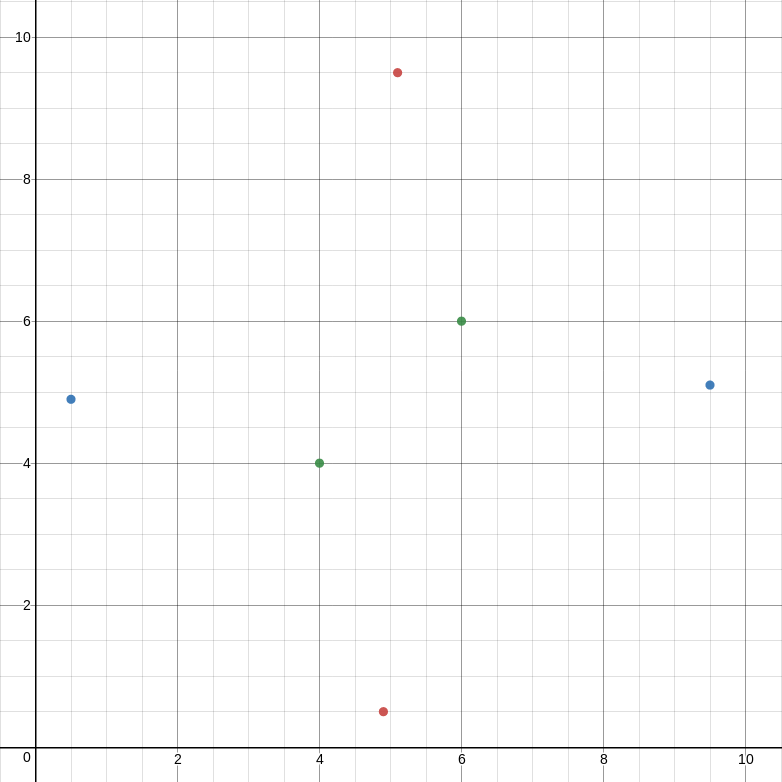
\includegraphics[scale=0.3]{cpopce}
\end{center}
It's clear here that the two green points are the closest together, but the algorithm would have returned either the pair of red points or the pair of blue points.\\\\
Let's try to come up with a divide and conquer algorithm to solve this problem. We can start by partitioning $\mathcal{P}$ into two sets, $\mathcal{P}_L$, and $\mathcal{P}_R$, of cardinality $\frac{n}{2}$. This gives us three possible outcomes:
\begin{enumerate}
	\item The closest pair of points is in $\mathcal{P}_L$
	\item The closest pair of points is in $\mathcal{P}_R$
	\item The closest pair of points has one point in $\mathcal{P}_L$, and the other point in $\mathcal{P}_R$
\end{enumerate}
To summarize this idea so far, we have the algorithm\\\\
---------------------------------------------------------------------------------------------------------
DCPair2D($\mathcal{P}$)\\
	\hspace*{7mm} find the point $q$ with the median $x$-coordinate\\
	\hspace*{7mm} partition $\mcal{P}$ into $\mcal{P}_L$, and $\mcal{P}_R$\\\\
	\hspace*{7mm} find the closest pair of points in $\mcal{P}_L$\\
	\hspace*{7mm} find the closest pair of points in $\mcal{P}_R$\\
	\hspace*{7mm} find the closest pair of points with one point in $\mcal{P}_L$ and the other in $\mcal{P}_R$\\\\
	\hspace*{7mm} return the pair from the above 3 with the smallest distance between them\\
---------------------------------------------------------------------------------------------------------\\
The recursive formula for this algorithm is given by
\[T(n) = 2\x T\Big(\frac{n}{2}\Big) + O(n^2)\]
The $O(n^2)$ term comes from the work needed to compare all $\frac{n}{2}$ points in $\mcal{P}_L$ with all $\frac{n}{2}$ points in $\mcal{P}_R$. $\big(\frac{n}{2} \times \frac{n}{2} = \frac{n^2}{4}$ comparisons.\big) Therefore, by the master theorem, the running time is $O(n^2)$.\\\\
This isn't any better than exhaustive search because there's a bottleneck step where we compare the points in $\mcal{P}_L$ with those in $\mcal{P}_R$. Indeed we're pretty much just doing exhaustive search but on only $\frac{n}{2}$ elements. With this in mind, let's try to slim this step down. Note that since we've solved both the left and right sub-problems, there's a minimum pairwise distance $\de$, given by
\[\de = \min(\de_L, \de_R)\]
for which the distance between the closest two points will not exceed, even if the two points are not in the same partition. Therefore, when looking for pairs of points with one point in each partition, we only need to look for points within $\de$ of the dividing line! From now on we will denote the set of points within $\de$ of the dividing line by $\mcal{P}_M$. This trick does work, but not trivially, so it has to be proved.\\\\
\lem Let $p_i \in \mcal{P}_L$, and let $p_j \in \mcal{P}_R$. If $d(p_i, p_j) \leq \de$ then $\{p_i, p_j\} \subseteq \mcal{P}_M$.\\\\
\proo WLOG assume that $p_i \notin \mcal{P}_M$. Then $d(p_i, p_j)\ \gt\ \de$. Similarily, if $p_j \notin \mcal{R}_M$. Then $d(p_i, p_j)\ \gt\ \de$. Thus if the pair of points is not within one of the two original sub-problems, it must be contained within $\mcal{P}_M$.
\qed\\\\
Let's implement this trick in the last algorithm we wrote up.\\\\
---------------------------------------------------------------------------------------------------------
DCPair2D($\mathcal{P}$)\\
	\hspace*{7mm} find the point $q$ with the median $x$-coordinate\\
	\hspace*{7mm} partition $\mcal{P}$ into $\mcal{P}_L$, and $\mcal{P}_R$\\\\
	\hspace*{7mm} find the closest pair of points in $\mcal{P}_L$\\
	\hspace*{7mm} find the closest pair of points in $\mcal{P}_R$\\
	\hspace*{7mm} find the closest pair of points in $\mcal{P}_M$\\\\
	\hspace*{7mm} return the pair from the above 3 with the smallest distance between them\\
---------------------------------------------------------------------------------------------------------\\
There's still a problem. $\mcal{P}_M$ can possibly contain all (or most) of the points! This means that our algorithm can $still$ take $\Omega(n^2)$ time to measure the distances between the points in $\mcal{P}_L \cap \mcal{P}_M$, and the points in $\mcal{P}_R \cap \mcal{P}_M$. Once again, however, this was fortunately not all for nothing. Since $\mcal{P}_M$ covers only a narrow band of the $x$-axis, we'll consider the area of the plane within $\de$ of the dividing line (i.e. the area pf $\mcal{P}_M$.) Suppose we divide this area into small squares of size $\frac{\de}{2}$ then we have the following lemma:\\\\
\lem No two points from $\mcal{P}$ will lie within the same square of width $\frac{\de}{2}$.\\\\
\proo WLOG take two points in a square in $\mcal{P}_L$. Then their pairwise distance $d$ is
\[d \leq \sqrt{\Big(\frac{\de}{2}\Big)^2 + \Big(\frac{\de}{2}\Big)^2} = \frac{\de}{\sqrt{2}}\ \lt\ \de\]
which is a contradiction as $\de$ is the smalles distance between two points.
\qed\\\\
\thm Let $p_i \in \mcal{P}_L$, and let $p_j \in \mcal{P}_R$. If $d(p_i, p_j) \leq \de$ then $p_i$, and $p_j$ have at most 10 points between them in $\mcal{P}_M$ with respect to their $y$-ordering.\\\\
\proo WLOG suppose that $p_i$ is below $p_j$ in the $y$-order. Then $p_j$ is in the same row of squares as $p_i$, or it is somewhere in the next two higher rows, or else they won't be within $\de$ of eachother (a contradiction). Therefore we are working in a rectangle that is at most three rows of squares high and four columns of squares wide. By the previous lemma we can have at most one point in any square and therefore in our $4 \times 3$ rectangle there can be at most 12 points. Thus, by choosing the the points on either extreme of the $y$-ordering of our rectangle, there can be at most 10 points between.
\qed\\\\
This result implies that the idea underlying the algorithm from the 1D case can be applied after all! We just have to tweak it slightly so as to look for points that are 11 apart rather than just adjacent, i.e. we'll have to calculate at most $11n$ pairwise distances rather than at most $n-1$. Thus we either find a pair of points in $\mcal{P}_M$ closer than $\de$ or we don't, but if we don't then we can conclude that no such pair of points exists, and we can do so in $O(n)$ time!\\\\
Let's update our algorithm to reflect this.\\\\
---------------------------------------------------------------------------------------------------------
DCPair2D($\mathcal{P}$)\\
	\hspace*{7mm} find the point $q$ with the median $x$-coordinate\\
	\hspace*{7mm} partition $\mcal{P}$ into $\mcal{P}_L$, and $\mcal{P}_R$\\\\
	\hspace*{7mm} find the closest pair of points in $\mcal{P}_L$\\
	\hspace*{7mm} find the closest pair of points in $\mcal{P}_R$\\
	\hspace*{7mm} find the closest pair of points in $\mcal{P}_M$ using the (updated) 1D algorithm\\\\
	\hspace*{7mm} return the pair from the above 3 with the smallest distance between them\\
---------------------------------------------------------------------------------------------------------\\
Now that we've gotten the bottleneck step down to $O(n)$, the new recurrence relation for this algorithm is
\[T(n) = 2\x T\Big(\frac{n}{2}\Big) + O(n)\]
where the $O(n)$ term comes from finding the median with respect to the $x$-coordinates (using algorithm from previous lecture), partitioning $\mcal{P}$, finding $\mcal{P}_M$ and applying the 1D algorithm. Thus, by the master theorem, the time complexity of this algorithm is $O(n\x \log n)$. (If you think about it, the new most expensive step is just sorting the points in $\mcal{P}_M$ with respect to the $y$-coordinates! If you don't think that's hella cool then you have no soul.)\\\\
Like most divide and conquer algorithms, this one is correct and the proof follows immediately from strong induction, where the proof that the base cases are correct follows from the proofs of the above various lemmas and theorems.
\newpage
%%%%%%%%%%%%%%%%%%%%%%%%%%%%%%%%%%%%%%%%%%%%%%%%%%%%%%%%%%%%%%%%%%%%%%%%

\section{Graph Algorithms}
\subsection{The Generic Search Algorithm}
Suppose we want to search a graph to determine whether there exists a path between a root node $r$ and some other node in the graph. Then we get the following algorithm:\\\\
---------------------------------------------------------------------------------------------------------
Search($r$)\\
	\hspace*{7mm} put $r$ into a bag\\
	\hspace*{14mm} while the bag is not empty\\
	\hspace*{21mm} remove a node $v$ from the bag\\
	\hspace*{21mm} if $v$ is unmarked\\
	\hspace*{28mm} mark $v$\\
	\hspace*{28mm} for each arc $(v, w)$\\
	\hspace*{35mm} put $w$ into the bag\\
---------------------------------------------------------------------------------------------------------\\
Where we say a new vertex (and therefore a path to that new vertex) is discovered when it's marked. We can write this algorithm in a bit more `formal' pseudo-code as such:\\\\
---------------------------------------------------------------------------------------------------------
Search($r$)\\
	\hspace*{7mm} set $\mcal{B} := \{r\}$\\
	\hspace*{14mm} while $\mcal{B} \neq \emp$\\
	\hspace*{21mm} let $v \in \mcal{B}$\\
	\hspace*{21mm} set $\mcal{B} \leftarrow \mcal{B} \setminus \{v\}$\\
	\hspace*{21mm} if $v$ is unmarked\\
	\hspace*{28mm} mark $v$\\
	\hspace*{28mm} for each arc $(v, w)$\\
	\hspace*{35mm} set $\mcal{B} \leftarrow \mcal{B} \cup \{w\}$\\
---------------------------------------------------------------------------------------------------------\\
Note that this algorithm allows multiple copies of the same node to be put into the bag. This $could$ pose a problem as it would require our algorithm excecute superfluous steps to terminate. We can get around this by putting edges into the bag instead of nodes. Let's update our pseudo-code to reflect this:\\\\\\\\\\\\\\\\
---------------------------------------------------------------------------------------------------------
Search($r$)\\
	\hspace*{7mm} set $\mcal{B} := \{(r, *)\}$\\
	\hspace*{14mm} while $\mcal{B} \neq \emp$\\
	\hspace*{21mm} let $(u, v) \in \mcal{B}$\\
	\hspace*{21mm} set $\mcal{B} \leftarrow \mcal{B} \setminus \{(u, v)\}$\\
	\hspace*{21mm} if $v$ is unmarked\\
	\hspace*{28mm} mark $v$\\
	\hspace*{28mm} set $p(v) \leftarrow u$\\
	\hspace*{28mm} for each arc $(v, w)$\\
	\hspace*{35mm} set $\mcal{B} \leftarrow \mcal{B} \cup \{(v, w)\}$\\
---------------------------------------------------------------------------------------------------------\\
Where $(r, *)$ is some pseudo-edge and $p(v)$ is the parent of $v$.
\subsubsection{Time Complexity}
We search every edge out of $v$ only once (when $u$ is first marked). The edge is added to the bag once and removed from the bag once. Thus the time complexity is $O(m)$ (where $m$ is the cardinality of the edge set.)
\subsubsection{Validity}
\thm Let $G$ be a connected, undirected graph. The generic search algorithn finds every vertex in $G$.\\\\
\proo We must show that every vertex is marked by the algorithm. We will do this by induction on the smallest number $k$ of edges in a path from the vertex to the root.\\
Base Case: $k=0$. Then $v$ is the root node $r$, but $r$ is marked by the algorithm.\\
Induction Hypothesis: Assume any vertex $v$ that has a path of $k-1$ or fewer edges to the root $r$ is marked.\\
Inductive Step: Assume there exists a path $P$ with $k$ edges from $v$ to $r$. i.e.
\[P = \{v = v_k, v_{k-1}, \dots, v_1, v_0 = r\}\]
Then there is a path $Q$ with $k-1$ edges from $u = v_{k-1}$ to $r$. i.e.
\[Q = \{u = v_{k-1}, \dots, v_1, v_0 = r\}\]
By our induction hypothesis $u$ is marked. After we mark $u$ we pace the edges incident to it in the bag. Therefore the edge $(u, v)$ is added to the bag. Thus when ($u, v$) is removed from the bag we will mark $v$ if it is not marked already.
\qed
\subsubsection{Search Trees}
Note that after running this algorithm, each non-root vertex has exactly one predecessor.\\\\
\thm Let $G$ be a connected, undirected graph. Then the predecessor edges form a tree rooted at $r$.\\\\
\proo We will prove this by induction on the number $k$ of marked vertices.\\
Base Case: $k=1$. The root vertex $r$ is the first one marked. Trivially, this forms a tree.\\
Induction Hypothesis: Assume the predecessor edges for the first $k-1$ marked vertices form a tree rooted at $r$.\\
Inductive Step: Let $v$ be the $k^{th}$ vertex to be marked. Assume that $v$ was marked when the edge $(u, v)$ was removed. Then $u = p(v)$. But $(u, v)$ was added to the bag when we marked vertex $u$. Therefore $u$ is in the set $S$ of the first $k-1$ vertices to be marked. By the induction hypothesis, the predecessor edges for $S$ form a tree $T$ rooted at $r$. Thus $T \cup (p(v), v)$ is a tree rooted at $r$ on the first $k$ marked vertices.
\qed\\\\
\thm For any vertex $v$, the path from $v$ to $r$ given by the search tree $T$ of predecessor edges is a shortest path.
\subsubsection{The Bag}
The bag is just shorthand for ``some data structure''. In this algorithm, the bag can be any data structure we want but our choice has some important consequences. Specifically, for the graph search algorithm we really want to use one of three data structures, each of which will give a distinct algorithm:
\begin{enumerate}
	\item Queue: The generic search algorithm becomes Breadth-First Search
	\item Stack: The generic searcg algorithm becomes Depth-First Search
	\item Priority Queue: The generic search algorithm becomes a Minimum Spanning Tree algorithm
\end{enumerate}
\subsection{Breadth-First Search}
Breadth-First search is an implementation of the generic search algorithm using a queue as the data structure (the bag.) Because we use a queue, edges are added in the order of their distance from $r$. The vertices are then marked in order of their distance from $r$.
\subsubsection{Breadth-First Search \& Bipartite Graphs}
\thm Let $G$ be a graph. Then $G$ is bipartite if and only if it contains no odd-length cycles.\\\\
\proo ($\imply$) Assume $G$ contains as a subgraph an odd-length cycle $C$. Let
\[C := \{v_0, v_1, \dots, v_{2k}\}\]
WLOG assume $v_0 \in Y$. Then
\[v_0 \in Y \imply v_1 \in X \imply v_2 \in Y \imply v_3 \in X \dots \imply v_{2k} \in Y\]
but $(v_0, v_{2k}) \in E$. Thus $v_0 \in Y \imply v_{2k} \in X$, a contradiction. Thus $G$ is not bipartite.\\
($\Leftarrow$) Assume $G$ contains no odd-length cycles. Then select an arbitrary root vertex $r$ and run the BFS algorithm. We want to show that if $G$ contains no odd-length cycles we can find two sets $X$, and $Y$ such that each edge goes only between $X$ and $Y$. Recall that for every edge ($u, v$) we have that $u$, and $v$ are either in the same layer or are in adjacent layers. Now set
\[X := \bigcup_{\ell \text{ odd}} S_{\ell} \text{, and, } Y := \bigcup_{\ell \text{ odd}} S_{\ell}\]
where $S$ is a set of nodes in the layer of a BFS-generated search tree, and $\ell$ is the level of the node form the root. We claim that this choice of $X$, and $Y$ gives a bipartite graph. Suppose that for each non-tree edge ($u, v$), that $u$, and $v$ are in adjacent layers. Assume that there exists a non-tree edge $(u, v)$ with $u$, and $v$ in the same layer. Let $z$ be the closest common ancestor of $u$, and $v$ in the search tree $T$ from $u$ to $v$; let $Q$ be the part in $T$ from $v$ to $z$. Since $u$, and $v$ are in the same layer $|P| = |Q|$. But then the cycle $C = P \cup Q \cup (u, v)$ has an odd number of edges, so $(u, v)$ can't exist, a contradiction.
\qed
\subsection{Depth-First Search}
Running the generic search algorithm but using a stack as our bag gives depth-first search. An interesting property of depth-first search is that it partitions the edges of an undirected graph into two types:
\begin{enumerate}
	\item Tree edges: Predecessor edges in the DFS tree $T$
	\item Back edges: Edges where one endpoint is an ancestor of the other endpoint in $T$
\end{enumerate}
we cannot have edges of the following type:
\begin{enumerate}
	\setcounter{enumi}{2}
	\item Cross edges: Edges where neither endpoint is an ancestor of the other in $T$
\end{enumerate}
\ \\
We can also define depth-first search recursively as such:\\\\\\\\\\\\\\
---------------------------------------------------------------------------------------------------------
RecursiveDFS($r$)\\
	\hspace*{7mm} mark $r$\\
	\hspace*{7mm} for each edge ($r, v$)\\
	\hspace*{14mm} if $v$ is unmarked\\
	\hspace*{21mm} set $p(v) \leftarrow r$\\
	\hspace*{21mm} RecursiveDFS($v$)\\
---------------------------------------------------------------------------------------------------------\\
\subsubsection{Ancestral Edges Theorem}
\thm Let $T$ be a depth-first search-generated tree in an undirected graph $G$. Then for each edge ($u, v$), either $u$ is an ancestor of $v$ in $T$, or $v$ is an ancestor of $u$.\\\\
\proo WLOG assume that $u$ is marked before $v$. Consider the time $u$ is marked during RecursiveDFS($u$). In RecursiveDFS($u$), the algorithm examines every arc incident to $u$. This leads to two cases:\\
Case 1: $v$ is unmarked when RecursiveDFS($u$) examines $(u, v)$. Then RecursiveDFS($u$) sets $p(v) \leftarrow u$. Therefore $(u, v)$ is a tree edge.\\
Case 2: $v$ is marked when the algorithm examines $(u, v)$. But $v$ must have been marked after $u$, so it was marked during RecursiveDFS($u$). Thus we have a series of vertices $\{u = w_0, w_1, \dots, w_{\ell -1}, w_{\ell} = v\}$ where $p(w_k) = w_{k-1}$. Therefore $u$ is an ancestor of $v$ in $T$ and is thus a back edge.
\qed
\ \\\\
\cor Let $T$ be a DFS tree in an undirected graph $G$. Then every non-tree edge is a back edge.
\subsubsection{Previsit \& Postvisit}
We can add a clock to the RecursiveDFS($r$) algorithm to record when we visit a vertex for the first time (previsit) and when we visit a vertex for the last time (postvisit). Let's update our recursive algorithm to include this.\\\\\\\\\\\\\\\\\\\\\\\\
---------------------------------------------------------------------------------------------------------
clock $\leftarrow 0$\\
RecursiveDFS($r$)\\
	\hspace*{7mm} mark $r$\\
	\hspace*{7mm} pre($r) \leftarrow$ clock\\
	\hspace*{7mm} clock++\\
	\hspace*{7mm} for each edge ($r, v$)\\
	\hspace*{14mm} if $v$ is unmarked\\
	\hspace*{21mm} set $p(v) \leftarrow r$\\
	\hspace*{21mm} RecursiveDFS($v$)\\
	\hspace*{7mm} post($r) \leftarrow$ clock\\
	\hspace*{7mm} clock++\\
---------------------------------------------------------------------------------------------------------\\
To visualize this imagine that a caterpillar is crawling along the graph like so:\\\\
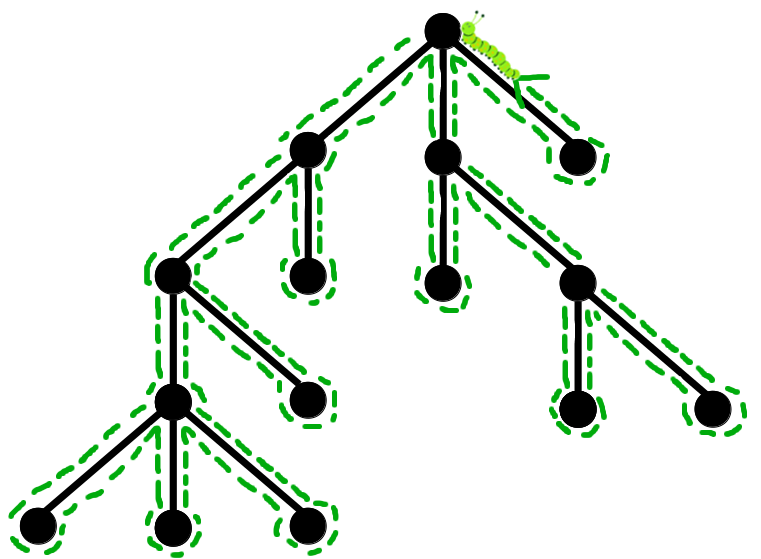
\includegraphics[scale=0.5]{cattree1}
\ \\
The clock records the first time the caterpillar visits a node and the last time the caterpillar visits a node. Then, let the black number be the clock on the previsit, and let the blue number be the clock on the postvisit. We get this
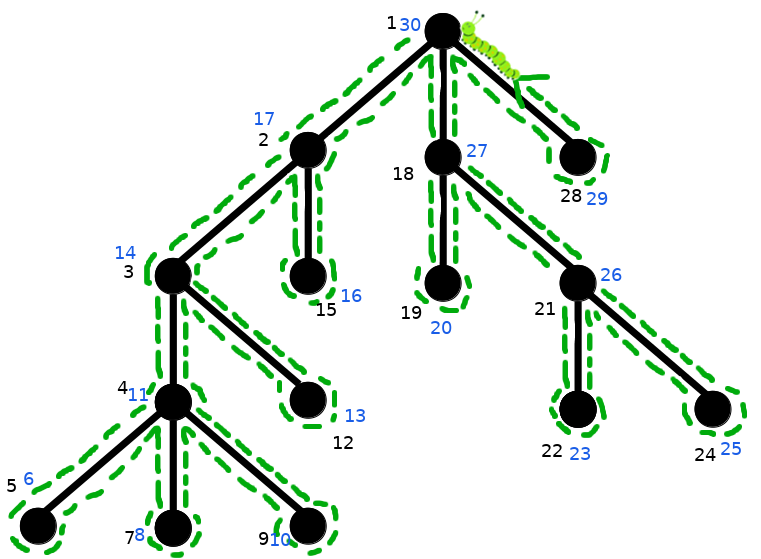
\includegraphics[scale=0.5]{cattree2}
\ \\
Note that pre($v$) is the time that the caterpillar arrives at the subtree rooted at $v$, and post$(v)$ is the time when the caterpillar leaves that subtree.\\\\
Depth-first search expores one subtree of the tree at-a-time. This means that we can represent each subtree as an interval over $\R$. More strongly, the set of intervals is laminar (for every pair of intervals, $I_1, I_2$, either $I_1$, and $I_2$ are disjoint, or one is a subset of the other.)
\subsubsection{Postvisit Times}
For an arc $(u, v)$ the following always hold:
\begin{enumerate}
	\item Tree arcs: post($v)\ \lt$ post($u$)
	\item Forward arcs: post($v)\ \lt$ post($u$)
	\item Backward arcs: post($u)\ \lt$ post($v$)
	\item Cross arcs: post($v)\ \lt$ post($u$)
\end{enumerate}
Note that only for backward arcs is post($u)\ \lt$ post($v$). This is a useful result.
\subsubsection{Directed Acyclic Graphs}
\thm A directed graph $G$ is acyclic if and only if depth-first search produces no backward arcs.\\\\
\proo ($\imply$) Let DFS give a backward arc ($u, v$). By definition $u$ is a descendant of $v$ in the DFS tree $T$. Therefore there exists a path $P$, given by $P = \{v = v_0, v_1, \dots, v_k =u\} \in T$. But then $P \cup (u, v)$ is a directed cycle in $T$, a contradiction.\\
($\Leftarrow$) Assume DFS gives no backward arcs. Suppose there is a directed cycle $C = \{v_0, v_1, \dots, v_k, v_0\} \in T$. Then, as there are no backward arcs we have that post($v_0$) $\gt$ post($v_1$) $\gt$ post($v_2$) $\gt\ \dots\ \gt$ post($v_k$) $\gt$ post($v_0$), a contradiction.
\qed\\\\
\cor We have an $O(m)$ algorithm to test whether the graph is acyclic.\\\\
\proo Run DFS and check for backward arcs.
\subsubsection{Topological Orderings}
A directed graph has a ``Topological Ordering" if the vertices can be ordered such that every arc is from right to left.\\\\
\thm A directed graph $G$ has a topological ordering if and only if DFS produces no backward arcs.\\\\
\proo ($\imply$) If DFS produces a backward arc then $G$ contains a cycle $C$. Let the cycle $C = \{v_0, v_1, \dots, v_k, v_0\}$, where WLOG $v_0$ is the leftmost vertex of the cycle in the order. But then the arc $(v_0, v_1)$ goes from left to right, a contradiction.\\
($\Leftarrow$) Assume DFS gives no backward arcs. Then for every arc $(u, v)$, we have that post($u$) $\gt$ post($v$). Thus, if we place each vertex $v$ at coordinate post($v$) on the $x$-axis, then every arc goes from right to left and hence $G$ has a topological ordering.
\qed\\\\
\cor We have an $O(m)$ algorithm to test whether or not we have a topological ordering.\\\\
\cor A directed graph is acyclic if and only if it has a topological ordering.
\subsubsection{Disconnected Graphs \& Strongly Connected Components}
For disconnected undirected graphs, a depth-first search from a vertex $r$ will find the entire component containing the vertex $r$. Therefore, if we want to discover the entire graph, not just the component containing $r$, we must run DFS from another vertex (in a different component).\\\\
In a directed graph, a subgraph $S$ is said to be strongly connected if for every vertex pair $u$, $v \in S$, there exists a directed path from $v$ to $u$ and vice versa. DFS can be used to decompose a directed graph into its strongly connected components very quickly.\\\\
\thm There is an $O(m)$ algorithm to find stromngly connected components of directed graphs.
\newpage

%%%%%%%%%%%%%%%%%%%%%%%%%%%%%%%%%%%%%%%%%%%%%%%%%%%%%%%%%%%%%%%%%%%%%%%%

\section{Greedy Algorithms}
Greedy algorithms are a class of algorithms characterized by how they make locally optimal choices at each step. They have a few properties:
\begin{itemize}
	\item They're fast!
	\item They're usually very simple!
	\item They're easy to code!
	\item They rarely work!
\end{itemize}
Thus for this topic in the course the goal is to understand some basic (working) greedy algorithms along with some basic techniques and when such techniques can succesfully be applied.
\subsection{The Task Scheduling Problem}
Suppose a firm receives a set $J$ of $n$ job orders from some customers, but the firm can only process one order at once. Suppose the job of customer $i$ will take $t_i$ units of time to complete. Assume each customer wants their job done as quickly as possible (and will pay accordingly.)\\\\
Assume the firm processes the jobs in order $\{1, 2, \dots, n\}$. Then the wating time of customer $\ell$ will be
\[w_{\ell} = \sum_{i = 1}^{\ell} t_i\]
Under the assumption that the customers will pay according to time, the firm wants to minimize the sum of the waiting times. That is, they want to minimize
\[\sum_{\ell = 1}^{n}w_{\ell} = \sum_{\ell = 1}^{n}\sum_{i = 1}^{\ell}t_i\]
We'll use a greedy approach to solve this problem:\\\\
---------------------------------------------------------------------------------------------------------
Schedule(J)\\
	\hspace*{7mm} sort the list of orders in non-decreasing order of their completion time\\
	\hspace*{7mm} schedule the jobs in this order\\
---------------------------------------------------------------------------------------------------------\\
Unfortunately, unlike divide and conquer algorithms that generally work, and where most of the proofs follow directly from strong induction (requiring only the base cases be verified), greedy algorithms don't work in general and thus have to be proved in more creative ways. Let's now prove the task scheduling algorithm works.\\\\
\proo Let the algorithm schedule the tasks in the order $\{1, 2, \dots, n\}$. Assume there is a better schedule $\mcal{S}$. Then there must be a pair of jobs $i, j$ such that
\begin{enumerate}
	\item Job $i$ is (WLOG) scheduled immediately before job $j$ by $\mcal{S}$.
	\item Job $i$ is longer than job $j$. In other words, $t_i\ \gt\ t_j$.
\end{enumerate}
This implies that exchanging jobs $i$, and $j$ leads to a more optimal schedule $\hat{\mcal{S}}$. Observe that after exchanging the two jobs the waiting time for all the other jobs remains the same (draw a picture if you need to convince yourself.) That is,
\[\hat{w}_k = w_k, \forall k \neq i, j\]
but obviously
\[\hat{w}_i + \hat{w}_j\ \lt\ w_i + w_j\]
a contradiction. Thus $\mcal{S}$ was the optimal solution.
\qed\\\\
The runtime of this algorithm is $O(n \log n)$ as the only real step is sorting the list of jobs by length.
\subsection{The Interval Selection Problem (Class Scheduling)}
Suppose there is one classroom and as set $I = \{1, 2, \dots, n\}$ of $n$ classes that want to use the room. Suppose each class $i \in I$ has a start time $s_i$, and a finish time $f_i$. Our goal is to book as many classes into that room as possible (in a certain period of time) but no more than one class can use the room at once. Let's try using a greedy algorithm to solve this problem. There's a couple different possibilities we can try:
\begin{enumerate}
	\item First start: Choose the class that starts first and iterate over the remaining non-conflicting classes
	\item Shortest duration: Select the class that is the shortest and then iterate over the remaining non-conflicting classes
	\item Minimum Conflict: Find the course that conflicts with the fewest other courses and iterate over the remaining non-conflicting classes
	\item First finish: Choose the class that finishes first and iterate over the remaining non-conflicting courses.
\end{enumerate}
\ \\
But do any of these actually work? Let's see.\\\\\\\\\\
Does first start work? Nope. Consider the example:\\\\
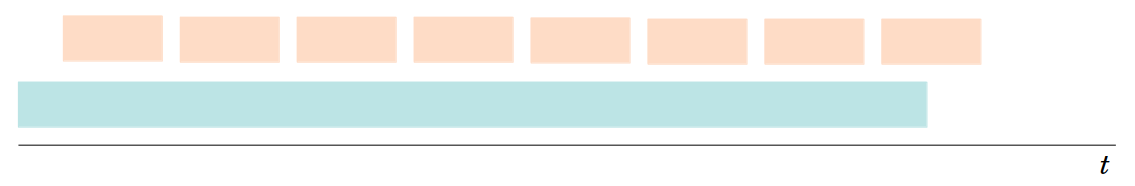
\includegraphics[scale=0.3]{ce1.png}\\
Note that that algorithm would select the blue interval where the eight orange intervals would be the optimal solution.\\\\
How about shortest duration? Nope. Consider the following:\\\\
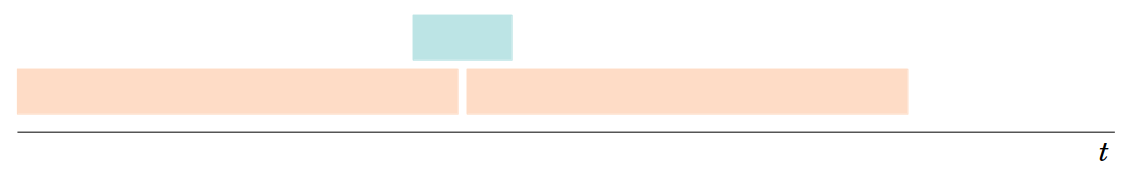
\includegraphics[scale=0.3]{ce2.png}\\
This algorithm would select the blue interval where the two orange intervals would be the optimal solution.\\\\
What about minimum conflict? Nope.\\\\
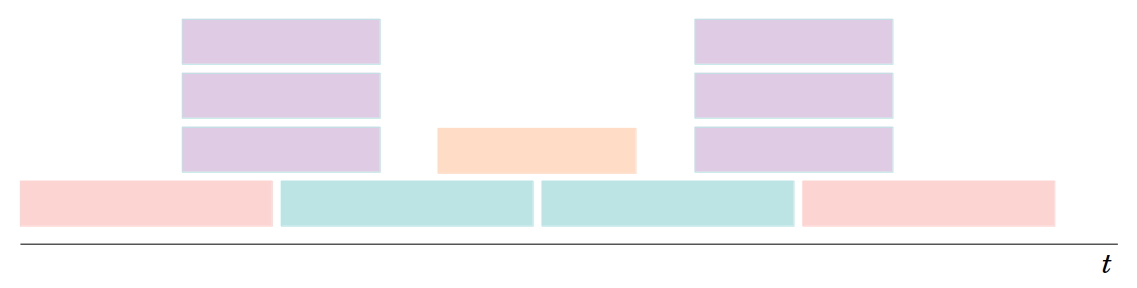
\includegraphics[scale=0.3]{ce3.png}\\
This algorithm would select the orange interval because it only conflicts with the two blue intervals, and then two of the purple intervals, but the blue intervals plus the red intervals along the bottom is the optimal solution even though the red intervals each conflict with the three purple intervals, and the blue intervals each conflict with four intervals.\\\\
First finish? Yep this one works. First we'll write down the pseudo-code algorithm and then we'll prove that it works.\\\\\\\\\\\\\\\\\\\\
---------------------------------------------------------------------------------------------------------
FinishFirst($I$)\\
	\hspace*{7mm} sort the classes by their finish time in non-decreasing order\\
	\hspace*{7mm} initialize the set $S := \emp$ to be the set of scheduled classes\\
	\hspace*{7mm} while $I \neq \emp$\\
	\hspace*{14mm} let $i$ be the lowest index class in $I$\\
	\hspace*{14mm} set $S \leftarrow S \cup \{i\}$ and set $I \leftarrow I \setminus \{i\}$\\
	\hspace*{14mm} for each class $j \in I$\\
	\hspace*{21mm} if $s_i\ \lt\ f_i$\\
	\hspace*{28mm} set $I \leftarrow I \setminus \{i\}$\\
	\hspace*{7mm} return $S$\\
---------------------------------------------------------------------------------------------------------\\
Before we prove the algorithm we need some help from a lemma\\\\
\lem Let $c$ be the class with the earliest finish time. Then there is an optimal solution that contains $c$.\\\\
\proo Recall the classes are indexed such that $f_1 \leq f_2 \leq \dots \leq f_n$. Then take an optimal solution $\mcal{S}$ and assume that $c \in \mcal{S}$. Let $i$ be the lowest index in $\mcal{S}$. We claim that $\mcal{S} \setminus \{i\} \cup \{c\}$ is a feasible allocation of maximum size. This follows as $f_i \leq s_j$ for any $j \in \mcal{S} \setminus \{i\}$. But $f_1 \leq f_i \leq s_j$ so $c$ doesn't conflict with any class in $\mcal{S} \setminus \{i\}$. Therefore $\mcal{S} \setminus \{i\} \cup \{c\}$ is feasible with cardinality equal to $|\mcal{S}|$.
\qed\\\\
We can now prove that the algorithm works.\\\\
\proo We'll proceed by induction on the cardinality of the optimal solution.\\
Base Case: Let $|\opt(I)|$ = 1. Then the algorithm outputs $c$ and this is trivially an optimal solution.\\
Induction Hypothesis: If $|\opt(I)| = k$ then the algorithm outputs an optimal solution.\\ 
Inductive Step: Let $|\opt(I)| = k+1$. Then the algorithm outputs $\{c\} \cup \text{FirstFinish}(I\setminus k)$. But by the previous lemma there exists an optimal solution $\hat{\mcal{S}}$ containing $c$. Thus $\hat{\mcal{S}}\setminus \{I\}$ is an optimal solution for the subproblem $I \setminus X$ $\imply |\opt(I)| = k$. But then by our induction hypothesis, the algorithm gives an optimal solution to the sub-problem $I \setminus X$ $\imply |\text{FirstFinish}(I \setminus X)| = k \imply |\{c\}\cup\text{FirstFinish}(I \setminus X)| = k+1$. Thus the algorithm outputs an optimal solution.
\qed\\\\
There are at most $n$ iterations, and it takes $O(n)$ time to find a class that finishes first. Therefore the runtime is $O(n^2)$. With better implementation, we can get the runtime down to $O(n \log n)$.
\subsection{Dijkstra's Shortest Path Alorithm}
\subsection{Huffman Codes}
\subsection{Minimum Spanning Tree Problem}
\subsubsection{Prim's Algorithm}
\subsubsection{Bor$\mathring{\text{u}}$vka's Algorithm}
\subsubsection{Reverse-Delete Algorithm}
\subsection{Clustering}
\subsection{Set Cover Problem}
\subsection{Matroids}
\newpage

%%%%%%%%%%%%%%%%%%%%%%%%%%%%%%%%%%%%%%%%%%%%%%%%%%%%%%%%%%%%%%%%%%%%%%%%

\section{Dynamic Programming}
\subsection{Fibonacci Numbers}
\subsection{The (Weighted) Interval Selection Problem}
\subsection{Knapsack Problem}
\subsection{Humpty Dumpty Problem}
\subsection{Bellman-Ford Algorithm}
\subsection{RNA Secondary Structure}
\subsection{Sequence Alignment}
\subsection{All-Pairs Shortest Paths}
\subsection{Independent Set on a Tree}
\newpage

%%%%%%%%%%%%%%%%%%%%%%%%%%%%%%%%%%%%%%%%%%%%%%%%%%%%%%%%%%%%%%%%%%%%%%%%

\section{Network Flows}
\subsection{Ford-Fulkerson Algorithm}
\subsection{Max Flow - Min Cut Theorem}
\subsection{Model Extensions}
\subsection{Bipartite Matching}
\subsection{Applications of Network Flows}
\subsection{Maximum Capacity Augmenting Path Algorithm}
\newpage

%%%%%%%%%%%%%%%%%%%%%%%%%%%%%%%%%%%%%%%%%%%%%%%%%%%%%%%%%%%%%%%%%%%%%%%%

\section{Data Structures}
\subsection{Priority Queues \& Heaps}
\subsection{Hashing}
\subsection{String Matching}
\subsection{Binary Search Trees}
\subsection{Data Structure for Disjoint Sets}
\subsection{Segment Trees}
\newpage

%%%%%%%%%%%%%%%%%%%%%%%%%%%%%%%%%%%%%%%%%%%%%%%%%%%%%%%%%%%%%%%%%%%%%%%%

\end{document}